\chapter{Ideas2d}
\section{Introduction}
\paragraph{}
Pour travailler sur Stample, j'avais besoin d'apprendre Scala.
Suite aux informations, tutoriels que j'ai suivies durant mon stage dans le but d'améliorer ma programmation  fonctionnelle. J'ai décidé de développer une page web personnelle pour mettre en valeur ce que j'ai appris.
\subparagraph{}
Au départ, l'idée consistait à écrire le contenu du rapport en HTML5 et l'héberger en ligne puis de l'imprimer, mais cela n'était pas possible vu que la page peut contenir des secrets profesionnels. 
\subparagraph{}
Sur ma page web personnelle Ideas2d\footnote{http://ideas2d.com/moncef/home.php}, un tutoriel intéressant pour les débutants en Scala.
Ce chapitre donne une idée générale sur Scala, vous trouverez plus de détailles sur ma page web.
\section{Contexte de Scala}
\paragraph{}
En 1996, James Gosling a conçu JAVA 1.0 avec Sun Microsystems.
Java a remporté plusieurs victoires : le débat du « write once/run everywhere », la gestion de la mémoire, une plateforme d'entreprise, un écosystème open-source énorme.
\subparagraph{}
Martin Odersky, qui n'est moins que l'inventeur du langage Scala. Il a effectué dans d'autres travaux de recherche scientifiques, langages de programmation (Pizza, GJ, Funnel langage ect...) et compilateurs. Cela lui a donné une reconnaissance dans ce domaine.
\subparagraph{}
Ce langage est conçu à  Ecole polytechnique fédérale de Lausanne en 2003, sa dernière version est Scala 2.10.\newline
Le nom Scala vient du besoin d'un langage "Scalable" qui passe l'innovation à l'échelle, multi-paradigme (Programmation concurrente, Programmation fonctionnelle, Programmation Acteur, ect...). Scala peut être vu comme un métalangage.
\section{Caractéristiques de Scala}
\subsection{Higher order functions}
\paragraph{}
Ce sont des fonctions qui prennent en paramètre d'autres fonctions.
Il est très utilisé dans les programmes Scala.
\newline
\textit{Exemple : conp[A,B,C](f:A=>B,g:B=>C):A=>C=x=>g(f(x))}
\subsection{Hiérarchie Scala}
Dans Scala tout est objet, la racine présentée par la classe Any comme "Object" en JAVA.
Les deux grands sous-classes sont "AnyRef", supertype de tous les types références (Scalaobject, Java classes, ect...);
"AnyVal", supertype de tous types de valeur (Int, Float, String, ect...).
En descendant dans la hiérarchie en trouve la class Nothing, elle hérite de tous les autres classes.

\begin{figure}[H]
        \centering
                \centering
                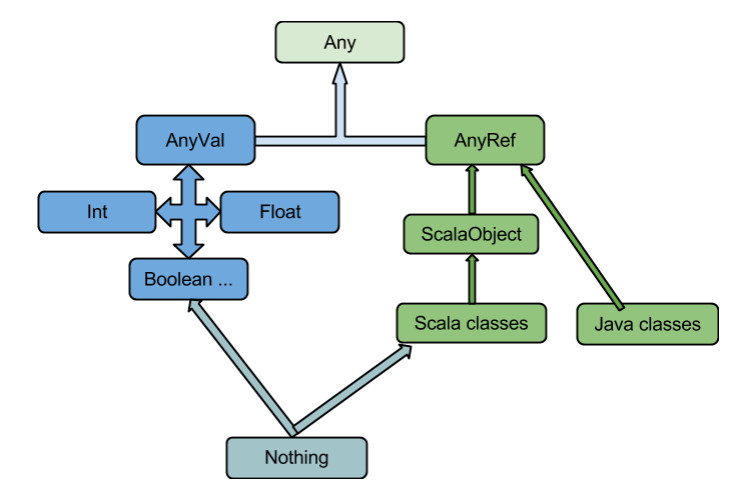
\includegraphics[width=10cm,height=8cm]{Hierarchie.png}
                \caption{Hiérarchie des classes Scala}
                \label{fig:Hiérarchie des classes Scala}
       
\end{figure}
\subparagraph{}
Techniquement Scala mélange la programmation orientée objet et fonctionnelle. Les deux styles de programmation ont des forces complémentaires quand il s'agit de l'évolutivité. Il tourne sur la machine virtuelle JAVA. Parmis ces points forts, il est compatible avec les libréries JAVA.
Scala est statiquement et fortement typé, c'est à dire qu'on déclare une variable et on l'affecte à une chaine de caractère. Elle sera automatiquement de type "String".
\newline
\textit{Exemple : val name="Moncef" <=> val name:String="Moncef"}

\subsection{Collections}
Il y a plusieurs concepts intéressants en Scala qu'on peut trouver dans autres langages de programmation fonctionnelle "Immutable DataStructures":
\begin{itemize}
\item \textbf{Map} : une collection pair de (clé/valeur). Toute valeur peut être récupérée en fonction de sa clé. Les clés sont uniques dans le Map, mais les valeurs n'ont pas besoin d'être unique.
\item \textbf{Option} : un conteneur de zéro ou un élément de type donné. Une "Option[T]" peut être soit un "Some[T]" ou un objet "None". \textit{Exemple : val x = Map("one" -> 1, "two" -> 2, "three" -> 3)}
\item \textbf{List} : une collection contenant des éléments de même type.   \textit{Exemple : val x = List(1,2,3,4,2)}
\item \textbf{Set } : une collection ne contient pas des duplications. \textit{Exemple : var x = Set(1,3,5,7)}
\end{itemize}
\section{Classes \& Objets}
\subsection{Classes}
\paragraph{}
Une classe est un modèle pour les objets. Une fois que vous définissez une classe, vous pouvez créer des objets à partir du modèle de classe avec le mot-clé "new".\newline
\textit{Exemple : class Person (val name:String)\newline 
val moncef=new Preson("Moncef")\newline
println(moncef.name)}
\subsection{Objets Singleton}
\paragraph{}
Scala est plus orientée objet que Java, parce que en Scala nous ne pouvons pas avoir des membres statiques. Au lieu de cela, Scala possède des objets uniques. Un singleton est une classe qui peut avoir qu'une seule instance 'objet'. Vous créez singleton à l'aide du mot-clé "object" au lieu de mot-clé "class". Puisque vous ne pouvez pas instancier un objet singleton, vous ne pouvez pas passer des paramètres au constructeur principal.
\textit{Exemple : object Person \{ def hello(p:Person)=println(s"Ahoy \$p.name !")\}\newline
Person.hello(moncef)}
\subsection{Trait}
\paragraph{}
Les Traits similaire à des interface en Java sont utilisés pour définir les types d'objets en spécifiant la signature des méthodes prises en charge. Scala permet également les traits d'être partiellement implémentés. Les traits Scala, et à l’inverse des interfaces de Java, peuvent avoir des champs et implémenter des méthodes.\newline
\textit{Exemple :    \newline
 trait ImageInfo\{
\newline
val image: Image
\newline
      def ImageInfo :String = image.name
\newline
\}
\newline
    trait ComputeAvgScore
\newline
    trait AnotherOne
}
\newline
\textit{
  class Image extends ImageInfo with ComuteAvgScore with AnotherOne\{
  \newline
      val name="Moncef"
  \newline\}}

\section{Pattern Matching}
\paragraph{}
Pattern Matching similaire au Switch case est le deuxième élément le plus largement utilisé de Scala, après "Higher order function". Scala fournit un grand soutien pour pattern matching pour le traitement des messages.
\subparagraph{}
Un pattern match comprend une séquence d'alternatives, chacune commençant par le cas de mots clés. Chaque solution comprend un motif et une ou plusieurs expressions, qui sera évalué si le motif correspond. Un symbole flèche => sépare le motif sur les expressions.
\section{Résumé}
\paragraph{}
Dans ce chapitre, j'ai essayé de donner une idée générale sur le langage. Pour plus de détails et d'exemples vous pouvez consulter Ideas2d. 
La pratique et les exercices sont les seuls moyens pour avoir la spécificité de ce langage.
La prochaine section se focalise sur la solution développée pour le login sur Stample.







